\chapter{Desenvolvimento da Aplicação}

Neste capítulo descrevemos os conceitos, análises e ferramentas
utilizadas pela equipe TGT para o desenvolvimento do porduto Lixt,
incluindo os requisitos do projeto, as tecnologias utilizadas, e a
arquitetura e a modelagem do produto.
Isto é apresentado para que se possa estabelecer parâmetros e métricas
que guiarão o desenvolvimento e a entrega final do projeto.

\section{Arquitetura}

Com base na análise do projeto, e nos requisitos que foram levantados
como necessários, a arquitetura cliente-servidor é plausível como
modelo para o produto que pretendemos entregar.
Esta arquitetura é composta por duas aplicações distintas:
\begin{itemize}
\item Uma aplicação \gls{frontend}, focada na interação com o usúario
  e apresentação de dados de uma forma agradável e intuitiva. Esta
  aplicação será implementada em JavaScript, com o \gls{framework} React
  Native, e disponibilizada para as plataformas iOS e Android.
\item Uma aplicação \gls{backend}, que será responsável por tratar os
  dados coletados no \gls{frontend} e disponibilizar as informações
  que serão mostradas aos usuários. Como esta aplicação requer uma
  lógica de servidor, estabilidade e ampla disponiblidade, esta
  aplicação será implementada em Java, com uso do \gls{framework} Spring
  Boot, que abstrai a criação de um servidor.
\end{itemize}
Podemos ver na \autoref{fig:cli-srv} uma respresentação desta
arquitetura.

\begin{figure}[h]
  \centering
  \caption{Arquitetura Lixt}
  \label{fig:cli-srv}
  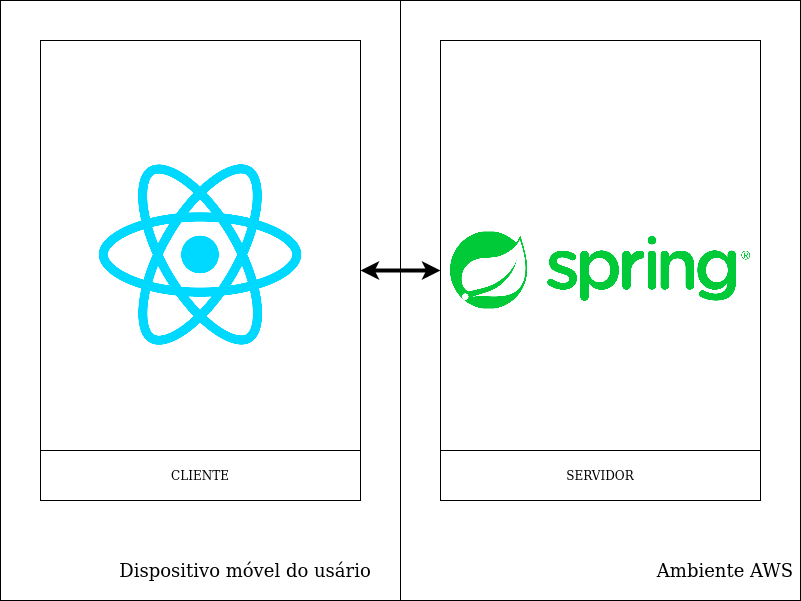
\includegraphics[scale=0.4]{lixt}
\end{figure}

A comunicação entre estes serviços será feita com o uso do protocolo
\label{sig:https}\hyperlink{s:http}{HTTPS}, que permite a aplicação
cliente realizar chamadas ao servidor através de urls, seja para
buscar informações para apresentar ao usuário ou postar informações
coletadas dele. O \gls{framework} Spring, além de abstrair a implementação
da lógica de um servidor, implementa \emph{listeners} para estas urls,
auxiliando a criação de pontos na aplicação do servidor focados na
comunicação com a aplicação cliente.

O uso do protocolo HTTPS oferece alguamas vantagens a aplicação
\gls{frontend}, que não precisa esperar uma solicitação ao
\gls{backend} ser finalizada antes de realizar outras solicitações,
aumentando a repsonsividade da aplicação cliente. Para além disso,
quando combinada ao modelo \label{sig:rest}\gls{REST} na
construção da \label{sig:API}\gls{API}, o protocolo HTTP
oferece meios eficientes para que as aplicações se comuniquem.

Como plataforma de servidor, o serviço AWS será utilizado, uma vez que
é oferecida de maneira gratuita para a realização deste projeto, e nele
serão armazenadas algumas instâncias da aplicação \gls{backend}.
Esta redundância é necessária como forma de garantir a estabilidade do
sistema, de forma que sempre haja alguma disponível para o
processamento de novas requisições, e, em caso de falha numa delas, o
serviço não seja interrompido aos usuários.

%%% Local Variables:
%%% mode: latex
%%% TeX-master: "../../desenho"
%%% End:


\section{Escopo do Projeto}

Lixt é um aplicativo para gerenciamento de listas de compras compartilhadas ou não.

O aplicativo vai seguir a dinâmica de uso abaixo:
\begin{enumerate}
	\item O usuário cria uma lista de compras e insere todos os itens antes da compra;
	\item O usuário inicia um carrinho de compras quando chega ao mercado, nesse momento ele tem a opção de importar para aquele carrinho os itens das listas que ele possui em aberto (que ainda não foram finalizadas), marcando quais listas ele deseja que sejam incluídas. Com o carrinho de compras ele poderá anotar os preços dos itens, riscá-los e ver o total gasto. Ao finalizar a compra as listas são atualizadas, e já aparecem riscados os itens que já foram comprados;
	\item Quando o usuário definir que uma lista não é mais relevante ele poderá deletar a lista ou desmarcar todos os itens, para reutilizar a lista.
\end{enumerate}

A seguir listamos as principais funcionalidades como uma lista de tópicos para facilitar a visualização de quais funcionalidades dependem de outras de forma hierárquica:

\begin{itemize}
	\item \textit{Login}:
		\begin{itemize}
			\item Criar conta;
			\item Redefinir senha;
		\end{itemize}
	\item Editar uma lista:
		\begin{itemize}
			\item Adicionar item:
				\begin{itemize}
					\item Definir nome;
					\item Definir quantidade;
					\item Definir unidade de medida (un. ml, L etc.);
					\item Definir medida;
					\item Adicionar uma categoria:
						\begin{itemize}
							\item Criar nova categoria;
						\end{itemize}
					\item Adicionar um comentário;
					\item Atribuir a um usuário (caso a lista tenha sido compartilhada e pelo menos um convite já tenha sido aceito);
				\end{itemize}
			\item Remover itens;
			\item Convidar pessoas para a lista (apenas quem criou a lista):
				\begin{itemize}
					\item Enviar convite:
						\begin{itemize}
							\item Acompanhar \textit{status} (aceito ou pendente);
							\item Remover convite;
						\end{itemize}
				\end{itemize}
			\item Deletar uma lista;
			\item Limpar uma lista;
		\end{itemize}
	\item Iniciar um carrinho de compras:
		\begin{itemize}
			\item Selecionar listas para compor o carrinho;
			\item Informar o mercado onde a compra será realizada (automaticamente através da localização, se não estiver habilitada será solicitado que o usuário insira o nome do mercado);
			\item Exibir o valor total do carrinho;
			\item Informar a quantidade que será efetivamente comprada naquele momento (o usuário pode ter planejado 10 unidades e apenas comprar 5 naquele momento);
			\item Riscar itens;
			\item Finalizar um carrinho de compras;
		\end{itemize}
	\item Ver estatísticas:
		\begin{itemize}
			\item Selecionar uma lista e ver o total gasto naquela lista ao longo do tempo em um gráfico de linha:
				\begin{itemize}
					\item Selecionar um dos pontos do gráfico e ver detalhes daquela lista;
				\end{itemize}
			\item Selecionar uma lista para ver um gráfico de pizza com os valores médios gastos por categorias naquela lista;
			\item Verificar histórico de preços de um item (tabela com nome do produto, quantidade, marca, preço, mercado e data da compra):
				\begin{itemize}
					\item Selecionar uma lista, dentro da lista selecionada selecionar o produto para ver o histórico;
				\end{itemize}
		\end{itemize}
\end{itemize}

Para o \textit{Minimum Viable Product} (\label{sig:mvp}\hyperlink{s:mvp}{MVP}) vamos implementar as seguintes funcionalidades, as demais ficarão para o próximo semestre:

\begin{itemize}
	\item \textit{Login}:
		\begin{itemize}
			\item Criar conta;
			\item Redefinir senha;
		\end{itemize}
	\item Criar lista de compra:
		\begin{itemize}
			\item Atribuir um nome;
			\item Atribuir uma descrição;
			\item Importar uma lista anterior;
		\end{itemize}
	\item Editar uma lista:
		\begin{itemize}
			\item Adicionar item:
				\begin{itemize}
					\item Definir nome;
					\item Definir quantidade;
					\item Definir unidade de medida (un., ml., L etc);
					\item Definir medida;
					\item Adicionar a uma categoria:
						\begin{itemize}
							\item Criar uma nova categoria;
						\end{itemize}
					\item Adicionar um comentário;
					\item Atribuir a um usuário (caso a lista tenha sido compartilhada e pelo menos um convite já tenha sido aceito);
				\end{itemize}
			\item Remover itens;
			\item Convidar pessoas para a lista (apenas quem criou a lista):
				\begin{itemize}
					\item Enviar convite:
						\begin{itemize}
							\item Acompanhar  status (aceito ou pendente);
							\item Remover convite;
						\end{itemize}
				\end{itemize}
			\item Deletar uma lista;
			\item Limpar uma lista;
		\end{itemize}
	\item Iniciar um carrinho de compras:
		\begin{itemize}
			\item Selecionar listas para compor o carrinho;
			\item Informar o mercado onde a compra será realizada (será solicitado que o usuário insira o nome do mercado manualmente);
			\item Exibir o valor total do carrinho;
			\item Informar a quantidade que será efetivamente comprada naquele momento (o usuário pode ter planejado 10 unidades e apenas comprar 5 naquele momento);
			\item Riscar itens;
			\item Finalizar o carrinho de compras.
		\end{itemize}
\end{itemize}

\subsubsection{Requisitos Funcionais}

Os requisitos funcionais dizem respeito às funcionalidade que o sistema deve ter. O Quadro \ref{reqFuncionais} lista os requisitos funcionais, suas dependências, a sigla e a prioridade de implementação.

\begin{quadro}[H]
\caption{Requisitos funcionais}
\begin{tabular}{|l|l|l|l|l}
\cline{1-4}
\textbf{Sigla} & \textbf{Descrição}                                                                                                                                                                                                                                               & \textbf{Prioridade} & \textbf{Dependências} &  \\ \cline{1-4}
RF01           & \begin{tabular}[c]{@{}l@{}}\textit{Login}: o usuário deve ser capaz de criar \\ sua conta no aplicativo, definir sua senha e \\ realizar o \textit{login} no sistema.\end{tabular}                                                                                                 & Alta                &                       &  \\ \cline{1-4}
RF02           & \begin{tabular}[c]{@{}l@{}}O sistema deve possibilitar que o usuário \\ crie suas listas de compras e possa atribuir um\\ nome, uma descrição e ter a opção de importar \\ uma lista existente.\end{tabular}                                                     & Alta                & RF01                  &  \\ \cline{1-4}
RF03           & \begin{tabular}[c]{@{}l@{}}Editar uma lista: Possibilita ao usuário o \\ gerenciamento dos itens da lista, como adicionar \\ itens, remover e enviar convites para a lista.\end{tabular}                                                                         & Alta                & RF02                  &  \\ \cline{1-4}
RF04           & \begin{tabular}[c]{@{}l@{}}Iniciar um carrinho de compras: permitir que o \\ usuário importe várias listas de compras, informe \\ o local da compra, o total gasto, quantidade de \\ itens a ser comprados, riscar itens e finalizar \\ o carrinho.\end{tabular} & Alta                & RF03                  &  \\ \cline{1-4}
RF05           & \begin{tabular}[c]{@{}l@{}}Ver estatísticas: ver o histórico de valores \\ pagos em uma lista ao longo do tempo, ver \\ os valores gastos por categorias em uma lista, \\ ver o histórico de preços de um determinado \\ item ao longo do tempo.\end{tabular}    & Média               & RF04                  &  \\ \cline{1-4}
\end{tabular}
\fonte{Os Autores}
\label{reqFuncionais}
\end{quadro}


\subsubsection{Requisitos Não Funcionais}

De maneira simplificada, os requisitos não funcionais não estão relacionados diretamente às funcionalidades do sistema, mas ao seu funcionamento de um modo geral, ou seja, como ele as funcionalidade serão executadas.

No Quadro \ref{reqNaoFuncionais} estão elencados os requisitos não funcionais, cada um com sua nomenclatura, categoria e descrição.

\begin{quadro}[H]
\caption{Requisitos Não funcionais}
\begin{tabular}{llll}
\cline{1-3}
\multicolumn{1}{|l|}{\textbf{Nomenclatura}} & \multicolumn{1}{l|}{\textbf{Descrição}}                                                                                                                                                                                                            & \multicolumn{1}{l|}{\textbf{Categoria}} &  \\ \cline{1-3}
\multicolumn{1}{|l|}{RNF01}                 & \multicolumn{1}{l|}{\begin{tabular}[c]{@{}l@{}}Criptografia das senhas: Por uma questão \\ de segurança as senhas não serão \\ armazenadas diretamente no banco, serão \\ criptografadas antes de serem armazenadas \\ como um \textit{hash}.\end{tabular}} & \multicolumn{1}{l|}{Segurança}          &  \\ \cline{1-3}
\multicolumn{1}{|l|}{RNF02}                 & \multicolumn{1}{l|}{\begin{tabular}[c]{@{}l@{}}Comunicação: A comunicação entre as \\ camadas da aplicação deverá ser feita utilizando \\ o protocolo HTTPS, para garantir a segurança \\ no envio dos dados através da rede.\end{tabular}}        & \multicolumn{1}{l|}{Segurança}          &  \\ \cline{1-3}
\multicolumn{1}{|l|}{RNF03}                 & \multicolumn{1}{l|}{\begin{tabular}[c]{@{}l@{}}Responsividade: O sistema deve exibir \\ corretamente os elementos da interface gráfica \\ nos mais variados tamanhos de celulares.\end{tabular}}                                                   & \multicolumn{1}{l|}{Usabilidade}        &  \\ \cline{1-3}
\multicolumn{1}{|l|}{RNF04}                 & \multicolumn{1}{l|}{\begin{tabular}[c]{@{}l@{}}Internacionalização: O sistema deverá suportar \\ dois idiomas (inglês e português) e suportar \\ que futuramente seja possível adicionar outros \\ idiomas.\end{tabular}}                          & \multicolumn{1}{l|}{Usabilidade}        &  \\ \cline{1-3}
\multicolumn{1}{|l|}{RNF05}                 & \multicolumn{1}{l|}{\begin{tabular}[c]{@{}l@{}}Escalabilidade: O sistema deverá ser projetado \\ para garantir que futuras melhoras e expansões \\ sejam possíveis.\end{tabular}}                                                                  & \multicolumn{1}{l|}{Desempenho}         &  \\ \cline{1-3}
\multicolumn{1}{|l|}{RNF06}                 & \multicolumn{1}{l|}{\begin{tabular}[c]{@{}l@{}}Disponibilidade: O sistema deverá estar disponível \\ aos usuários ininterruptamente\end{tabular}}                                                                                                  & \multicolumn{1}{l|}{Disponibilidade}    &  \\ \cline{1-3}
                                            &                                                                                                                                                                                                                                                    &                                         & 
\end{tabular}
\label{reqNaoFuncionais}
\fonte{Os Autores}
\end{quadro}

\section{Tecnologias Utilizadas}

As tecnologias que decidimos utilizar foram escolhidas a partir do conhecimento prévio da equipe, da curva de aprendizado e levando em consideração também o tamanho das comunidades que já a utilizam, visando um maior apoio e material de pesquisa.
Dito isso, escolhemos as seguintes tecnologias:

\subsection{Linguagens}

\subsubsection{Back-end}

Decidimos que a linguagem para o \gls{backend} seria o Java. A linguagem se adequa à nossa proposta e atende o paradigma de linguagem orientada a objetos do qual nos foi orientado a utilizar. 
A comunidade de Java é extensa e ativa, contribuindo com muitos materiais e recursos. Ainda podemos destacar que a utilização da linguagem previamente pelos integrantes da equipe também foi impactante na consolidação dessa decisão.

\subsubsection{Mobile}
Para o desenvolvimento da plataforma mobile decidimos utilizar o Javascript. A linguagem possui também uma comunidade ativa e uma variedade de materiais disponíveis e atualizados. Apesar de nem todos os integrantes terem tido contato prévio, por conta da facilidade de assimilação e necessidade de poucos recursos para a configuração do ambiente de desenvolvimento, optamos pelo Javascript.

\subsection{Frameworks e ORMs}

\subsubsection{Back-end}

Para o \gls{backend} decidimos utilizar o \gls{framework} Spring, usando a ferramenta Spring Boot que proporciona agilidade na criação das aplicações pois segue a filosofia de Convention over Configuration\cite{Devopedia2020}, nos poupando de depreender muito tempo nas configurações. Não obstante, a \gls{framework} facilita o desenvolvimento pois nos propicia a utilização de módulos que julgarmos necessários (como Spring MVC e Spring Data JDBC). Além disso, há uma gama vasta de materiais para consultarmos.
Como ferramenta \gls{ORM} decidimos usar o Hibernate pela consolidação dele no mercado e o uso amplo em aplicações Java que necessitam de mapeamento relacional dos dados. Por conta da quantidade de modelos da aplicação, julgamos necessário utilizar uma ferramenta que facilitasse esse processo. 

\subsubsection{Mobile}
Na aplicação mobile decidimos utilizar o \gls{framework} React-Native. Esta \gls{framework} gera aplicativos nativos, não necessita de muitos recursos e configurações para montar o ambiente de desenvolvimento e possibilita um conforto maior no desenvolvimento do código por ser uma \gls{framework} Javascript. Não obstante, também é uma \gls{framework} com larga quantidade de recursos para consulta além de uma comunidade muito ativa.

\subsection{Banco de dados}
O banco de dados que escolhemos foi o MySQL pois precisávamos para a nossa proposta de um banco de dados relacional e que fosse possível de ser hospedado na AWS. Verificamos que o MySQL cobria não apenas esses critérios mas também possui uma ferramenta gráfica (MySQL Workbench) que facilita a visualização e a operação do banco. Além disso os integrantes da equipe já tiveram experiências com a ferramenta anteriormente.

\subsection{Gerenciamento de tarefas}
Para o gerenciamento das tarefas optamos pela ferramenta Trello por ser gratuita, de fácil manuseio e visualização.
Além disso, o Trello figura entre as ferramentas que foram utilizadas com sucesso nos semestres anteriores durante o desenvolvimento de projetos.

\subsection{Versionamento}
Para o controle de versão do desenvolvimento da aplicação optamos pelo Git com repositório no Github. Esta escolha foi realizada devido à experiência prévia da equipe com a ferramenta e pela quantidade de recursos oferecidos pela plataforma na gestão do desenvolvimento de aplicações.
Para o versionamento do projeto utilizamos o Apache Subversion (SVN). Concentramos no repositório fornecido pelos professores todas as entregas previstas (incluindo as versões atualizadas dos códigos do repositório externo do Github).



%%% Local Variables:
%%% mode: latex
%%% TeX-master: "../proposta"
%%% End:


\section{Escalabilidade}

A escalabilidade da aplicação é sua capacidade de se adequar a um
amplo volume de requisições, mantendo a estabilidade do sistema e a
velocidade de respostas. Um sistema escalável está apto para responder
adequadamente nestes momentos, assim como liberar seus recursos em
momentos com poucas requisições.

Por se tratar de algo relativo ao processamento de requisições, a
escalabilidade diz respeito ao \gls{backend}, que centraliza os
pedidos dos usúarios. A camada cliente por outro lado, por focar
exclusivamente na lógica de visualização, e rodar em dispositivos
mobile, não exige tanta capacidade de processamento, e a
escalabilidade não é uma preocupação para esta camada.

Como foi mencionado, a aplicação \gls{backend} ficará armazenada na
plataforma Amazon AWS. Existe um processo da ferramenta de integração
contínua Jenkins para aumentar o número de instâncias ativas em
produção, e este processo será acionado em momentos com intenso volume
de requisições.


%%% Local Variables:
%%% mode: latex
%%% TeX-master: "../../desenho"
%%% End:


\section{Manutenibilidade da aplicação}

É fundamental para o desenvolvimento do projeto, tanto o previsto
quanto em avanços posteriores, que a aplicação atinja um nível adequado
de qualidade, e para tanto certos requisitos de manutenibilidade devem
ser estabelecidos.  Estes requisitos permitem estabelecer critérios
para medir o quanto o processo de desnvolvimento está de acordo com
boas práticas, e incentivam que estas práticas sejam seguidas.

\subsection{\emph{Logs}}

Como forma de monitorar a aplicação em tempo de execução,
especialmente na camada de servidor, \emph{logs} serão usados para
registrar o estado dos objetos. A ferramenta Log4j será usada, uma vez
que os membros da equipe já tem mais familiaridade com ela. Esta
ferramenta perimite o registro em diversos níveis, como
\begin{itemize}
  \em
\item info
\item debug
\item warn
\item error
\end{itemize}
e pode ser configurada para que apenas os dois últimos
sejam registrados no ambiente de produção. Desta forma a cada ponto de
falha da aplicação um log de nível apropriado será colocado para que
problemas sejam rapidamente identificados, analisados e resolvidos.

\subsection{Integração Contínua}

Visando manter o serviço sempre atualizado para o usuário, a
ferramenta de integração contínua Jenkins foi selecionada para a
implantação da aplicação \gls{backend} em produção. Ela permite a
configuração de tarefas, também chamada de \emph{jobs}, que facilitam
a implantação do sistema.

O diagrama \ref{fig:jenkins} ilustra o funcionamento da ferramenta:
\begin{enumerate}
\item uma instância dela, rodando no ambiente AWS tem acesso ao código no
github;
\item no momento do \gls{deploy}, a instância, rodando em uma máquina
  virtual cria um processo filho, que realiza o \emph{checkout} do
  código fonte no Github, executa testes e o \emph{build} da
  aplicação;
\item uma cópia deste \emph{build} é salva em uma máquina virtual
  secundária, como histórico das versões da aplicação;
\item pr fim, na máquina virtual final, onde o sistema será
  implantado, a imagem é copiada e iniciada.
\end{enumerate}
Vale notar que, quando o \emph{deploy} é realizado, uma instância só é
derrubada quando uma nova instância, de uma nova versão, está
plenamente operante.

\begin{figure}
  \centering
  \caption{Diagrama ilustrando o processo de \emph{deploy}.}
  \includegraphics[scale=0.50]{images/deploy}
  \label{fig:jenkins}
\end{figure}

Para o \gls{frontend}, no entanto, não existem ferramentas de
integração contínua, uma vez que as imagens do aplicativo mobile
precisam ser aprovadas pelas lojas de aplicativo. Contudo, ainda é
possível usar ferramentas de CI para a execução de testes e
verificação da integridade do código a cada nova versão.

\subsection{\emph{Code Conventions}}

As convenções de código são acordos internos ao equipe que visam
estandartizar a forma como os diversos integrantes do equipe produzem
seus códigos.  Elas visam facilitar o entendimento mútuo entre os
integrantes da equipe, de modo o estilo de progamação seja indistiguível
e independente de seus autores.  Geralmente, as convenções de código
estabelecem estilos para se organizar o código textualmente, isto é,
dizem respeito a forma como nomes de variáveis são escolhidas e
comentários são posicionados, por exemplo.

As convenções adotadas são baseadas na especificação da
\citeauthor{Oracle1997}, de 1997. Esta é comumente usadas para o
desenvolvimento na linguagem Java, e muito próxima do padrão adotado
em JavaScript, e vale destacar o seguintes pontos:
\begin{itemize}
\item Minimizar o uso de variáveis, funções e objetos globais.
\item As declarações globais estarão preferencialmente no início do arquivo.
\item Declarar as variáveis próximo do ponto onde elas serão inicializadas.
\item A indentação é de 4 espaços.
\item Linhas mais longas que 80 caracteres serão quebradas e
  indentadas a 8 espaços.
\item Pacotes e variáveis com nomes curtos, em \texttt{camelCase} e substantivos.
\item Classes e interfaces em \texttt{CamelCase} e substantivos.
\item Métodos em \texttt{camelCase} e verbos.
\item Constantes em \texttt{UPPER\_CASE}.
\end{itemize}

No entanto, especificamente para a linguagem Java,
\begin{itemize}
\item Classes e métodos devem ser documentados com um comentário na
  seguinte forma, uma vez que as IDEs reconhecem este formato e
  formatam o text na forma de \emph{pop-ups} quando o cursor está
  sobre uma referência a esta classe.
\begin{verbatim}
/**
 * Class ListService
 *
 * Implementar endpoints para as funcionalidades de lista.
 */
\end{verbatim}
\end{itemize}

No backend, a estrutura de pacotes vai ser bem dividida, tendo o pacote controller para os controllers e endpoints, mapper para os mappers. O model, service e repository de uma entidade ficarão no mesmo pacote cujo nome é o mesmo nome da entidade.

\subsection{\emph{Designs Patterns}}

Como padrões de projetos, serão usados 3 padrões amplamente utilizados pela comunidade de desenvolvimento: (I) Clean Code, (II) SOLID e (III) Gang Of Four. Esses 3 padrões podem ser utilizados tanto no backend quanto no frontend.

\subsubsection{\emph{Clean Code}}

O Clean Code é um conjunto de boas práticas para melhorar o entendimento do código, de modo que seja mais fácil sua leitura. Segue abaixo uma lista das principais boas práticas:

\begin{itemize}
	\item Nome Significativos para variáveis, classes, métodos, atributos e objetos, evitando abreviaturas desnecessárias e nomes não recorrentemente utilizados, sendo passíveis de busca.
	\item Evitar números mágicos, recomendando-se utilizar enums e constantes para que seja mais compreensível ao analisar o código.
	\item Evitar booleanos de forma implícita.
	\item Evitar condicionais negativos (por exemplo, uma função com nome "naoDevoExecutar()"), visto que dificulta a compreensão de código.
	\item Encapsular condicionais.
	\item Nunca comentar o óbio no código.
	\item Utilizar funções pequenas, tanto para melhorar a leitura quanto para respeitar os padrões do SOLID.
\end{itemize}

\subsubsection{\emph{SOLID}}

O SOLID é um acrônimo de 5 príncipios da Programação Orientada a Objetos, sendo fundamental para o desenvolvimento e manutenção de software.

\begin{itemize}
	\item \underline{\textbf{S}ingle Responsiblity Principle}: Uma classe deve ter apenas um motivo para mudar.
	\item \underline{\textbf{O}pen-Closed Principle}: Uma classe deve estar aberta para extensão, e fechada para modificação, recomendando sempre utilizar a herança e não modificar o código fonte original.
	\item \underline{\textbf{L}iskov Substitution Principle}: Uma classe derivada deve ser substituível por sua classe base.
	\item \underline{\textbf{I}nterface Segregation Principle}: Utilizar muitas interfaces específicas é melhor do que uma interface genérica.
	\item \underline{\textbf{D}ependency Inversion Principle}: Dependa de abstrações e não de implementações.
\end{itemize}

\subsubsection{\emph{Gang Of Four}}

O GoF (ou Gang of Four) se refere aos profissionais que criaram os 23 padrões de projetos, nos quais seus conceitos serão utilizados no desenvolvimento do Lixt.

Segue abaixo uma breve apresentação dos principais padrões utilizados:

\begin{itemize}
	\item \underline{Builder}: Será utilizado para criar instâncias legíveis de objetos complexos.
	\item \underline{Facade}: Encapsula regras de negócios complexas.
	\item \underline{Observer}: Observa e é capaz de reagir às mudanças de estado de um objeto.
\end{itemize}

\subsection{Testes}

Testes são uma ferramenta fundamental para o desenvolvimento da
aplicação, uma vez que garantem, em tempo de compilação, o
comportamento correto do aplicativo. Para além disso, testes tem um
papel de documentação, uma vez que encapsulam de forma breve o
comportamento esperado das classes e métodos produzidos, e podem ser
consultados em caso de dúvida quando ao uso destes. Este tipo de teste
é chamado de teste unitário, em oposição aos testes de integração, que
verificam o funcionamento da aplicação de ponta-a-ponta, isto é, a
partir de uma chamada a um endpoint, apenas os serviços externos são
mimetizados, garantindo o funcionamento correto de toda a aplicação.

Desta forma, a construção de testes, de ambos os tipos é de extrema
importância para a elaboração do projeto visando a sua
manutenibilidade, e será o primeiro passo de uma sprint, após o
planejamento, a construção de testes relevantes para a tarefa,
seguindo os princípios do TDD\cite{TDD}. Como as ferramentas de teste são
específicas de cada linguagem, cada camada da aplicação fará uso de
frameworks distintos.

O \gls{backend} será testado com o framework JUnit, fazendo uso da
biblioteca Mockito quando necessário simular comportamentos de objetos
que não são o alvo da suite de teste. Este framework ainda oferece
ferramentas para testar o banco de dados, ou melhor, testar a conexão
com o banco e verificar o comportamento das classes de acesso a ele.
Já os teste de \gls{frontend} serão feitos com a biblioteca Jest,
que auxilia a construção de testes unitários, e por se tratar de uma
\gls{GUI}, as interações de usuário devem ser simuladas também. Para tanto, a
biblioteca React Testing Library será usada.

%%% Local Variables:
%%% mode: latex
%%% TeX-master: "../../desenho"
%%% End:


\input{capitulos-desenvolvimento/section/segurança}

\section{Viabilidade Financeira}

O projeto de análise de viabilidade financeira consiste em averiguar a garantia de lucro sobre as despesas do projeto. Portanto, nesse projeto será descrito cada processo a fim de fazer essa verificação.

\subsection{Gerenciamento de Custos}

Nesse tópico, serão abordados temas de investimento inicial e de desenvolvimento do projeto, incluindo tópicos de análise de requisitos, desenvolvimento, manutenções e imprevistos.

\subsubsection{Análise de Requisitos e Desenvolvimento}

Para iniciar o projeto, é necessário fazer os primeiros planejamentos, elicitação de requisitos, abstrair e concretizar as primeiras ideias e fazer os primeiros planejamentos (diagramas, cronogramas e documentação). Logo após, o projeto chega na fase de desenvolvimento, onde é começado a se tornar real.

Contudo, o projeto não vai possuir nenhum custo de análise e implementação do sistema, devido ao fato de ser um projeto educacional.

\subsubsection{Manutenções}

Inevitavelmente, manutenções do sistema ocorrerão pós finalização do projeto e estar devidamente funcional em produção. Contudo, os custos de manutenções também não serão cobrados, devido a ser um projeto educacional.

\subsection{Custos de deploy e de Ambiente de Produção}

Nesse tópico, são apresentados os custos de manter o sistema funcional e disponível para os usuários. Desse modo, será feito uma previsão anual de cada plataforma utilizada:

\subsubsection{Frontend} 

Tendo em vista que o projeto é \textit{mobile} voltado para dispositivos Android, será publicado na PlayStore, estimando um valor de 25.00 USD anual. 

\subsubsection{Backend}

Inicialmente gratuito no Amazon EC2, sendo permitido 750h de instâncias por mês durante o período de 12 meses.

A partir do momento que for necessário grande porte, será indicado o plano Sob Demanda do Amazon EC2, que garante viabilidade econômica e estratégica (visto que o preço é calculado a partir do uso). 

Utilizando a calculadora da AWS e optando por um servidor Linux da instância t4g.micro com 1 vCPU e 1GiB, com armazenamento SSD de uso geral de 10GB, será custeado o valor de 7,52 USD mensalmente para operar o mês inteiro.

\subsubsection{Banco de Dados} 

Inicialmente gratuito no Amazon RDS, sendo permitido 750h de instâncias durante o período de 12 meses. O Amazon RDS possui suporte a vários \gls{sgbd}, incluindo o MySQL, que foi o \gls{sgbd} optado para desenvolver a aplicação Lixt.

A partir do momento que for necessário grande porte, será indicado o plano Sob Demanda do Amazon RDS, que garante viabilidade econômica e estratégica (visto que o preço é calculado a partir do uso).

Utilizando a calculadora da AWS e optando por um servidor da instância t2.micro de modelo Single-AZ OnDemand, com armazenamento SSD para cada instância de 10GB, será custeado o valor de 27,74 USD mensalmente para operar o mês inteiro.

\subsection{Medidas de Obtenção de Retorno Financeiro}

Para gerar uma receita positiva a fim de obter lucro, haverá duas formas principais de retorno financeiro:

\begin{itemize}
	\item \underline{Cobrança do aplicativo}: O aplicativo estará disponível gratuitamente na PlayStore, não gerando, portanto, retorno financeiro.
	\item \underline{Propaganda/Recomendação}: Será utilizado mediador de anúncio AdMob (responsável por conectar aplicações e anunciantes), onde o valor varia por visualizações de anúncios e cliques neles. Contudo, no próprio site do admob, é citado um caso no qual houve 300.000 downloads e arrecadava, através do AdMob, 100 USD por dia. \cite{GoogleAdMob}
\end{itemize}

A partir da calculadora do AdMob, estimando-se uma quantidade de 250 visitantes por dia, onde há 2 paginas visualizadas por visitante, sendo que a taxa de cliques em anúncios é 1\% e o custo do clique é 0.35 USD, o valor mensal será de 52.5 USD.

\subsection{Conclusão}

Concluindo que, ao utilizar os servidores de baixo porte detalhados acima, será desembolsado cerca de 35.00 USD por mês. Contudo, o valor calculador para 250 visitantes (estimando o valor com baixo engajamento) com os parâmetros detalhados arrecadará 52.5 USD, conseguindo custear os servidores e ainda garantindo margens de lucro.

Conforme o engajamento na aplicação for aumentando, será revisto os planos dos servidores para atender maiores níveis de requisições.


%%% Local Variables:
%%% mode: latex
%%% TeX-master: "../desenho"
%%% End:
